\section{Teori}

\subsection{LED-diode}

En lysdiode, eller lysemitterende diode (LED), er en halvlederkomponent som emitterer lys når den gjennomstrømmes av elektrisk strøm. Komponenten har to terminaler: anode (positiv) og katode (negativ). LED-dioden har samme grunnleggende egenskaper som en vanlig diode, ved at den leder strøm i én retning og sperrer i motsatt retning. I lederetningen har dioden lav motstand (ideelt null), mens den i sperreretningen har svært høy motstand (ideelt uendelig).

\begin{figure}[H]
\centering
\begin{circuitikz}
    \draw (0, 0) to[led] (3, 0);
\end{circuitikz}
\caption{Symbol for LED-diode}
\end{figure}

\noindent
I elektroniske kretser benyttes LED-dioder ofte som indikatorer, for eksempel som statuslys. LED-dioden har et typisk spenningsfall på omtrent 2 V ved nominell strøm, basert på databladverdier \cite{led-datasheet}. Dette benyttes videre i beregning av strøm gjennom dioden.

\subsection{Kondensator}

En kondensator er en passiv elektronisk komponent som lagrer elektrisk energi i et elektrisk felt. Den består av to ledende plater adskilt av et isolerende materiale, kalt et dielektrikum. Kondensatorens evne til å lagre ladning beskrives ved kapasitansen $C$, definert som forholdet mellom ladning $Q$ og spenning $V$:
\[
C = \frac{Q}{V}
\]

\noindent
Kapasitansen måles i farad (F), og bestemmes blant annet av plateareal, avstand mellom platene og egenskapene til dielektrikumet. I en elektrisk krets vil en kondensator motsette seg raske spenningsendringer, og har da en dynamisk sammenheng mellom strøm og spenning, hvor strømmen som går gjennom kondensatoren er bestemt av kapasitansen og endring i spenning:
\[
i(t) = C \frac{d v(t)}{dt}
\]

\noindent
Ved likestrøm (DC) vil den etter opplading fungere som en åpen krets, på grunn av ingen endring i spenning, mens den for vekselstrøm (AC) kan slippe signaler gjennom avhengig av frekvens, og oppføre seg som en kortslutting.

\begin{figure}[H]
\centering
\begin{circuitikz}
    \draw (0,0) to[C] (3,0);
\end{circuitikz}
\caption{Symbol for kondensator}
\end{figure}

\noindent
Kondensatorer benyttes blant annet til filtrering, kobling av signaler og som del av resonansretser, slik som i oscillatorer.


\subsubsection{Trimming}
En trimmerkondensator er en kondensator med variabel kapasitans, hvor kapasitansen kan justeres mekanisk, typisk ved hjelp av en skrue.

\begin{figure}[H]
\centering
\begin{circuitikz}
    \draw (0,0) to[variable capacitor] (3,0);
\end{circuitikz}
\caption{Symbol for trimmerkondensator}
\end{figure}

\noindent
Trimmerkondensatorer benyttes ofte til finjustering av resonansfrekvens i oscillator- og filterkretser.

\subsection{Spole}


\subsection{Transistor}

\subsection{NE555 timer}

\subsection{Antenne}


\subsection{Kretsanalyse}
I denne seksjonen presenterer vi kretsen, og gjør beregninger på den for å begrunne brettets oppbygning og plassering av komponenter.

\begin{figure}[H]
\centering
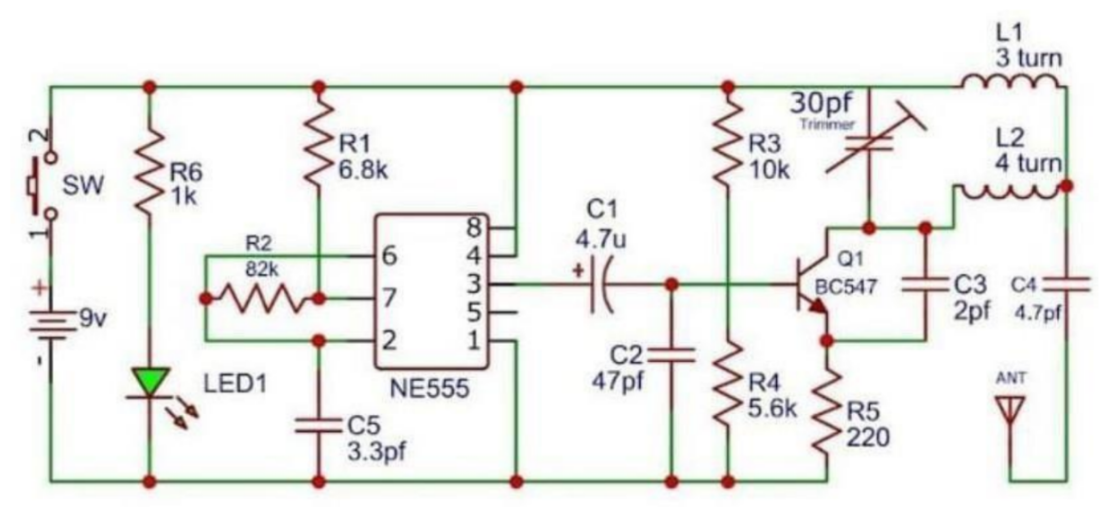
\includegraphics[width=0.9\textwidth]{Media/circuit.png}
\caption{Mobiljammerkretsen.}
\end{figure}

\noindent
Analyserer vi stegvis fra venstre ser vi et standard 9V batteri og en bryter. Bryteren bestemmer om kretsen er ''på'' eller ''av'', på grunn av at det er et bindeledd for strømvei. Dersom bryteren er på vil toppskinnen i kretsen ha en spenning 9V høyere enn bunnskinnen (jording). Grenen med $R_6$ og lysdioden $LED_1$ vil derfor indikere om kretsen er på eller ikke. Strømmen gjennom dioden vil være:
\begin{gather*}
    9\text{V} = V_{R6} + V_{LED} \\
    9\text{V} = I_{R6} \cdot R_6 + 2\text{V} \\
    7\text{V} = I_{R6} \cdot 1\text{k}\Omega \\
    I_{R6} = 7\text{mA}
\end{gather*}

\noindent
Dette er helt innafor ifølge datablad for LED-dioden, og den vil lyse nok for formålet sitt. Videre har vi NE555 timeren. I den aktuelle koblingen er pin 2 (trigger) og pin 6 (threshold) til NE555 koblet til samme node. Dette gjøres bevisst for å la begge inngangene overvåke spenningen over kondensatoren $C_5$.
\\[1em]
Når spenningen over kondensatoren er lavere enn $\frac{1}{3}V_{CC}$, aktiveres triggerinngangen (pin 2), og utgangen settes høy. Kondensatoren begynner da å lades gjennom motstandene $R_1$ og $R_2$. Når spenningen når $\frac{2}{3}V_{CC}$, aktiveres threshold-inngangen (pin 6), og utgangen settes lav. Samtidig kobles utladingstransistoren internt i NE555 (pin 7) til jord, slik at kondensatoren utlades gjennom $R_2$.
\\[1em]
Denne kontinuerlige vekslingen mellom opplading og utlading gjør at kretsen oscillerer, og NE555 opererer dermed i astabil modus. Frekvensen til oscillatoren bestemmes da av komponentverdiene for $R_1$, $R_2$ og $C_5$. For en RC-krets gjelder:
\[
V(t) = V_{CC} \left(1 - e^{-t / RC}\right)
\]